\chapter{Langlands纲领的几何重述之一：Galois表示}\label{L10}\lecturedate{2020/03/18}\sourcepage{80}
函数域情形中的Langlands纲领更为理想，部分原因在于这里可以使用一些尚不能用于数域的几何方法。因此，尝试以几何语言重述这一对应是很自然的。人们已经对任意域上的代数曲线，以及任意约化群完成了这样的重述，范围并不限于$\GL_n$。不过，遗憾的是，还没有向高维代数概形的相应推广。
\section{平展基本群}\label{L10S1}\idx{平展基本群}
在Galois表示一侧，希望把表示实现为代数曲线上的局部系统\znote{局部系统即局部常值层：每点附近都同构于常值层。拓扑或解析情形下，它与 $\pi_1(X,x)$ 的表示范畴等价，对应由沿道路的解析延拓（单值化）给出；平展情形下则由 $\widehat\pi_1(X,\overline x)$ 的连续表示刻画。正因如此，「Galois 表示 $\leftrightarrow$ 曲线上的局部系统」才能成为几何重述的出发点：表示论的对象被搬到了曲线 $X$ 上。[来源：nLab "local system"，\url{https://ncatlab.org/nlab/show/local+system}（Last revised 2025-04-10；2026-11-14 访问）。]}，亦即光滑层。首先，需要把Galois群$\Gal(F^{\mathrm{sep}}/F)$看成平展基本群\znote{平展基本群是拓扑基本群的代数替代物：对连通概形 $X$ 与几何点 $\overline x$，它由有限平展覆盖范畴上纤维函子 $\mathcal F_{\overline x}$ 的自同构群定义（见定义 1.6），因而自动是射有限群。其有限连续表示与 $X$ 上的有限平展覆盖一一对应，这就是 Grothendieck 的 Galois 理论；取 $X=\Spec k$ 时它退化为绝对 Galois 群 $\Gal(k^{\mathrm{sep}}/k)$。由于只用有限覆盖，它看不到路径，这与拓扑情形不同。[来源：nLab "fundamental group"，\url{https://ncatlab.org/nlab/show/fundamental+group}（Last revised 2025-09-04；2026-11-14 访问；另见本讲参考文献 Milne《Lectures on étale cohomology》）。]}。

回忆：对一个足够好的拓扑空间$X$及基点$x\in X$，基本群$\pi_1(X,x)$是$X$中以$x$为基点的闭路的同伦类所成的群，运算由路径复合给出。路径很容易形象地理解，但在代数几何中，无法直接找到适合的路径与同伦概念。因此，我们转而通过通用覆盖来描述基本群。

对道路连通、局部道路连通且半局部单连通的拓扑空间$X$，其\textbf{通用覆盖}$\widetilde X\to X$是连通、单连通的覆盖空间；其他单连通覆盖空间$E\to X$
\sourcepage{81}
均可通过$\widetilde X$分解，即下图交换：
\begin{figure}[H]\centering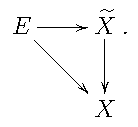
\includegraphics[width=0.1115\paperwidth]{images/L10-p081-cover.pdf}\end{figure}
$\widetilde X$存在，并且在同构意义下唯一。此时，通用覆盖$\widetilde X\to X$通过下式恢复基本群：
\begin{equation}\tag{1.1}\label{L10eq11}
\pi_1(X,x)\cong\operatorname{Aut}(\widetilde X/X).
\end{equation}
由\eqref{L10eq11}也可看出，只要通用覆盖存在，基本群的同构类型就不依赖于基点。
\originalnumber{1}
\begin{note}[L10S1O1]
拓扑空间$X$称为\textbf{半局部单连通}，是指每个点的每个邻域都含有一个子邻域，使子邻域中以该点为基点的闭路可以在$X$中缩到一点。这比每个邻域都含有单连通子邻域的条件弱。
\end{note}
\originalnumber{2}
\begin{example}\label{L10S1O2}
指数映射$\exp:\C\to\C^\times$，$a\mapsto e^{2\pi ia}$，是$\C^\times$的通用覆盖。因此，$\pi_1(\C^\times,x)\cong\operatorname{Aut}(\C/\C^\times)\cong\Z\varphi$，其中$\varphi:\C\xrightarrow{\sim}\C$，$a\mapsto a+1$。同时也可看到，指数映射不是代数映射。
\end{example}
% [Tutor Note: 原书 p81 的例 1.2 作 "is a universal covering of $\mathbb{A}^\times$"，但指数映射的靶是 $\C^\times$，下一句也写作 $\pi_1(\C^\times,x)$，故应为 $\C^\times$ 的通用覆盖；译文已按 $\C^\times$ 处理。]
在多数情形中，通用覆盖不是代数的；而且解析空间在Zariski拓扑下几乎从不是半局部单连通的。缺少代数通用覆盖时，构造基本群的代数类似物的方法，是考察有限平展覆盖\znote{有限平展覆盖是同时有限且平展的态射 $Y\to X$：有限保证几何纤维是有限集，平展则取代拓扑中「局部同构」的角色——它等价于相对微分消失（$\Omega^1_{Y/X}=0$）并配合适当的平坦性。合起来，$Y\to X$ 就是「无分支的有限覆盖」，其自同构群的逆极限给出平展基本群（见推论 1.9）。注意平展并非真正的局部同构，只是形式局部同构。[来源：nLab "etale morphism of schemes"，\url{https://ncatlab.org/nlab/show/etale+morphism+of+schemes}（Last revised 2026-07-03；2026-11-14 访问）。]}的自同构群所组成的逆系统。换言之，平展基本群都是射有限群。
\originalnumber{3}
\begin{definition}{射有限群及射有限完备化}\label{L10S1O3}\idx{射有限群}\idx{射有限完备化}
\textbf{射有限群}$\widehat G$是有限群逆系统$(G_n)$的逆极限，即$\widehat G=\varprojlim_nG_n$。若$G$为拓扑群，其\textbf{射有限完备化}为
\[G^\wedge:=\varprojlim_{\substack{U\triangleleft G\text{为开正规子群}\\{}[G:U]<\infty}}G/U.\]
\end{definition}
\sourcepage{82}
\originalnumber{4}
\begin{theorem}\label{L10S1O4}
拓扑群是射有限群，当且仅当它紧且全不连通\znoteplain{原书此处未写 Hausdorff，只假设拓扑群紧且全不连通；而射有限群按定义（有限离散群的逆极限）自动 Hausdorff 紧，若不加分离性假设，结论只在带 T0 分离公理时才成立，故通行表述通常写明 Hausdorff。阅读原书时须自行补上这一假设，正文按原书处理。（上下文推断，无外部依据）}。
\end{theorem}
一般地，给定概形$X$及几何基点$\overline x$，平展基本群$\widehat\pi_1(X,\overline x)$是射有限群，其有限连续置换表示对应于$X$上的有限平展概形。

平展态射有以下性质：
\begin{enumerate}
\item 平展性在基变换下保持。
\item 平展性在复合下保持。
\item 在交换图
\begin{figure}[H]\centering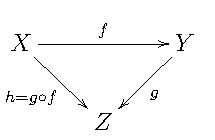
\includegraphics[width=0.1737\paperwidth]{images/L10-p082-etale.pdf}\end{figure}
中，若$g,h$平展，则$f$平展。由此可见，若$Z$连通，$h,g$有限平展，且$f$在某个几何纤维上诱导同构$X_z\cong Y_z$，则$f$为同构。
\item 有限平展态射是固有态射。
\item 平展态射局部可以表示成$\Spec B\to\Spec A$，其中
\[B\cong A[x_1,\ldots,x_n]/(f_1,\ldots,f_n),\]
且Jacobian行列式$\Delta=\det(\partial f_i/\partial x_j)$在$B$中可逆；反过来，这种局部表示给出平展态射。
\end{enumerate}
记$\mathrm{FET}/X$为$X$的有限平展覆盖范畴。对几何点$\overline x:\Spec\overline k\to X$，其中$\overline k$代数闭，有纤维函子$\mathcal F_{\overline x}:\mathrm{FET}/X\to(\mathrm{Sets})$，将$Y\to X$送到几何纤维的点集$F_{\overline x}(Y):=(Y\times_X\Spec\overline k)(\overline k)$。
\originalnumber{5}
\begin{definition}{函子的自同构}\label{L10S1O5}
设$\mathcal F:\mathcal C\to(\mathrm{Sets})$为小范畴$\mathcal C$上的函子。$\mathcal F$的一个自同构$\xi=(\xi_X)_{X\in\operatorname{Ob}(\mathcal C)}$，是
\sourcepage{83}
$\prod_{X\in\operatorname{Ob}(\mathcal C)}\operatorname{Aut}(\mathcal F(X))$中的元素，满足：对任意态射$f:X\to Y$，下图交换。
\begin{figure}[H]\centering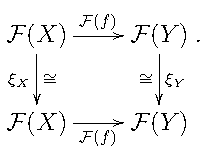
\includegraphics[width=0.1677\paperwidth]{images/L10-p083-functor.pdf}\end{figure}
因此，$\operatorname{Aut}(\mathcal F)\subset\prod_{X\in\operatorname{Ob}(\mathcal C)}\operatorname{Aut}(\mathcal F(X))$。
\end{definition}
% [Tutor Note: 原书 p83 定义 1.5 把自同构写作 $\xi=(\xi_X)_{X\in\operatorname{ob}(E)}$，其中 $E$ 应为上文的小范畴 $\mathcal C$（$\operatorname{ob}(E)$ 系排版笔误）；译文按 $\operatorname{Ob}(\mathcal C)$ 处理。]
\originalnumber{6}
\begin{definition}{平展基本群}\label{L10S1O6}
对连通概形$X$，定义其平展基本群为
\[\widehat\pi_1(X,\overline x):=\operatorname{Aut}(\mathcal F_{\overline x}),\]

\end{definition}
\originalnumber{7}
\begin{note}[L10S1O7]
对任意两个几何点$\overline x_1,\overline x_2$，有$\widehat\pi_1(X,\overline x_1)\cong\widehat\pi_1(X,\overline x_2)$。
\end{note}
注意，对$\mathrm{FET}/X$中的每个$Y\to X$，$\widehat\pi_1(X,\overline x)$作用于$F_{\overline x}(Y)$。对连通覆盖，若$|\operatorname{Aut}(Y/X)|=|F_{\overline x}(Y)|$，称$Y\to X$为\textbf{Galois覆盖}。
\originalnumber{8}
\begin{theorem}\label{L10S1O8}
若$Y$连通，则$\widehat\pi_1(X,\overline x)$在$F_{\overline x}(Y)$上传递作用。
\end{theorem}
\originalnumber{9}
\begin{corollary}\label{L10S1O9}
为连通Galois覆盖选取与$\overline x$相容的基点后，有
\[\widehat\pi_1(X,\overline x)\cong\varprojlim_{\substack{Y\to X\\\text{连通Galois覆盖}}}\operatorname{Aut}(Y/X).\]
\end{corollary}
\originalnumber{10}
\begin{example}\label{L10S1O10}
$n$次循环覆盖$\C^\times\to\C^\times$，$a\mapsto a^n$，是平展覆盖，其自同构群为$\Z/n\Z$。这些覆盖给出$\C^\times$的平展基本群$\widehat{\Z}=\varprojlim_n\Z/n\Z$。
\end{example}
\originalnumber{11}
\begin{example}\label{L10S1O11}
对任意域$k$，有$\widehat\pi_1(\Spec k,\overline k)=\Gal(k^{\mathrm{sep}}/k)$，其中$\overline k$为代数闭包，$k^{\mathrm{sep}}$为可分闭包。注意，有限扩张$L/k$可分，当且仅当$\Omega^1_{L/k}=0$。
\end{example}
\sourcepage{84}
\originalnumber{12}
\begin{example}\label{L10S1O12}
设$A$为完备离散赋值环，极大理想为$\mathfrak m$，剩余域$k\cong A/\mathfrak m$。则基变换给出范畴等价$\mathrm{FET}/\Spec A\simeq\mathrm{FET}/\Spec k$。若$\overline x:\Spec\overline k\to\Spec k$为几何点，其在$\Spec A$中的像记为$\overline y$，则
\[\widehat\pi_1(\Spec k,\overline x)\xrightarrow{\sim}\widehat\pi_1(\Spec A,\overline y).\]
\end{example}
\section{光滑层}\label{L10S2}\idx{光滑层}\idx{局部系统}
设$f:X'\to X$为连通概形之间的态射。基变换给出函子$\mathrm{FET}/X\to\mathrm{FET}/X'$。取$X'$的几何点$\overline x'$，令$\overline x=f(\overline x')$，则有射有限群的典范同态
\[f_*:\widehat\pi_1(X',\overline x')\to\widehat\pi_1(X,\overline x).\]
\originalnumber{1}
\begin{theorem}\label{L10S2O1}
设$X$为正规整Noether概形，函数域为$K$，泛点为$\eta\to X$。则典范映射
\[\Gal(K^{\mathrm{sep}}/K)\cong\widehat\pi_1(\Spec K,\overline K)\longrightarrow\widehat\pi_1(X,\overline\eta)\]
可以等同于商映射$\Gal(K^{\mathrm{sep}}/K)\to\Gal(K^{\mathrm{ur}}/K)$，其中$K^{\mathrm{ur}}$为由$X$上的有限平展覆盖所对应的扩张组成的最大处处非分歧代数扩张。因此，$\Gal(K^{\mathrm{ur}}/K)\cong\widehat\pi_1(X,\overline\eta)$。
\end{theorem}
可借助下面的正规化事实理解\eref{定理}{L10S2O1}。
\originalnumber{2}
\begin{lemma}\label{L10S2O2}
设$X$为正规整Noether概形，函数域为$K$。若$L/K$有限可分，则存在有限支配态射$Y\to X$，其中$Y$正规且整，函数域为$L$。此外，$Y\to X$平展当且仅当它非分歧\znoteplain{原书此引理既未假定正规化有限，也未限定 $X$ 为曲线：$Y$ 的存在需要 $X$ 为 Nagata 概形（正规曲线上自动成立），而「有限非分歧即平展」的等价通常也要求 $X$ 维数不超过 1 或该态射平坦。阅读时须自行补上相应假设，正文按原书处理。（上下文推断，无外部依据）}。
\end{lemma}
% [Tutor Note: 原书 p84 的引理 2.2 未提「正规化有限」与「$X$ 为正规曲线」这两项条件，译文原曾补足，现按原书回退，条件问题见上方译注。]
\eref{定理}{L10S2O1}使我们可以把$\Gal(K^{\mathrm{sep}}/K)$的处处非分歧表示看成$\widehat\pi_1(X,\Spec\overline K)$的表示。若$X$为复代数簇，还有如下比较定理。
\sourcepage{85}
\originalnumber{3}
\begin{theorem}{Grothendieck--Riemann存在定理}\label{L10S2O3}
设$X$为$\C$上局部有限型概形。把有限平展覆盖$Y\to X$送到其解析化$Y^{\mathrm{an}}\to X^{\mathrm{an}}$，给出范畴等价$\mathrm{FET}/X\simeq\mathrm{FET}/X^{\mathrm{an}}$。特别地，对复几何基点$\overline x$及相应解析点$x$，有
\[\widehat\pi_1(X,\overline x)\cong\pi_1(X^{\mathrm{an}},x)^\wedge.\]
\end{theorem}
回忆：若$X$为$\C$上的光滑射影曲线，则解析拓扑中$n$维复向量空间的局部常值层的同构类，与$\pi_1(X)$的$n$维表示的同构类一一对应。复流形解析拓扑中的局部常值层，也等价于带有全纯平坦联络的全纯向量丛。

代数几何中不能普遍使用解析拓扑，但存在类似物，即\textbf{平展拓扑}。概形$X$的平展拓扑是一种Grothen\-dieck拓扑。其中，“开集”为平展态射$U\to X$，覆盖为联合满射的态射族。$X$连通时，通过$\mathcal F\mapsto\mathcal F_{\overline x}$，有限平展局部常值层的范畴与$\widehat\pi_1(X,\overline x)$的有限连续作用范畴等价。

设$X$为$k$上的连通正规且几何连通概形，$\ell\ne\operatorname{char}(k)$，$E_\lambda$为$\Q_\ell$的有限扩张，$K$为$X$的函数域。
\originalnumber{4}
\begin{definition}{光滑$E_\lambda$层}\label{L10S2O4}
$X$上的\textbf{光滑$E_\lambda$层}\znote{光滑 $E_\lambda$ 层（lisse sheaf）就是 $E_\lambda$ 局部系统：它由 $\widehat\pi_1(X,\Spec\overline K)$ 的有限维连续 $E_\lambda$ 表示给出，秩即纤维 $V_{\mathcal F}$ 的维数。它与可构造层的关系是：光滑层在每个层上都局部常值、局部有限生成，因而是可构造层中最「局部平凡」的一类。系数取 $E_\lambda$（$\Q_\ell$ 的有限扩张）而非 $\Q_\ell$，是因为 $\ell$ 进表示的本征值一般只落在有限扩张中，取 $E_\lambda$ 后迹等不变量才落在 $E_\lambda$ 内。[来源：nLab "constructible sheaf"，\url{https://ncatlab.org/nlab/show/constructible+sheaf}（Last revised 2025-10-31；2026-11-14 访问；该条目较短，另见本讲参考文献 Milne《Lectures on étale cohomology》）。]}$\mathcal F$，亦称$E_\lambda$\textbf{局部系统}，是有限维连续$E_\lambda$表示
\[\rho_{\mathcal F}:\widehat\pi_1(X,\Spec\overline K)\to\GL(V_{\mathcal F}),\]
其中$V_{\mathcal F}$称为层的纤维，是有限维$E_\lambda$向量空间，即$V_{\mathcal F}=\mathcal F_{\Spec\overline K}$。$\mathcal F$的秩为$\operatorname{rk}(\mathcal F)=\dim_{E_\lambda}V_{\mathcal F}$。
\end{definition}
\sourcepage{86}
\section{单值表示}\label{L10S3}\idx{单值表示}\idx{外单值表示}
本节介绍通过平展基本群实现的一类Galois表示。

先看拓扑基本群上的单值作用。设$f:E\to X$为纤维化，固定基点$x\in X$及其上方的点$y\in E$。记$F_x$为$x$处的纤维，则$F_x\xrightarrow{\iota}E\xrightarrow f X$诱导同伦群长正合列
\[\begin{aligned}
\cdots\to\pi_1(F_x,y)\xrightarrow{\iota_*}\pi_1(E,y)\xrightarrow{f_*}\pi_1(X,x)\xrightarrow{\partial_y}\pi_0(F_x,y)\\
\xrightarrow{\iota_*}\pi_0(E,y)\xrightarrow{f_*}\pi_0(X,x)\to1.
\end{aligned}\]
假定$F_x$道路连通，并进一步假定$\pi_2(X,x)=0$，或者$\pi_1(F_x,y)$的中心平凡；则得到基本群的短正合列
\begin{equation}\tag{3.1}\label{L10eq31}
1\to\pi_1(F_x,y)\xrightarrow{\iota_*}\pi_1(E,y)\xrightarrow{f_*}\pi_1(X,x)\to1.
\end{equation}
对于$\sigma\in\pi_1(X,x)$，选择提升$\widetilde\sigma\in\pi_1(E,y)$，定义其对$\pi_1(F_x,y)$的外作用：
\[\rho(\sigma)(\gamma):=\widetilde\sigma\gamma\widetilde\sigma^{-1},\qquad\gamma\in\pi_1(F_x,y).\]
由于该元素属于\eqref{L10eq31}中$f_*$的核，它仍在$\pi_1(F_x,y)$中。
% [Tutor Note: 原书 p86 此处作 "since it is in the kernel of map $f_*$ in (??)"，交叉引用编号失效；按上下文应为 (3.1)，译文已按 \eqref{L10eq31} 处理。]$\rho(\sigma)$在
\[\operatorname{Out}(\pi_1(F_x,y)):=\operatorname{Aut}(\pi_1(F_x,y))/\operatorname{Inn}(\pi_1(F_x,y))\]
中的像不依赖于提升，仍记为$\rho(\sigma)$。称$\rho:\pi_1(X,x)\to\operatorname{Out}(\pi_1(F_x,y))$为$f:E\to X$在$x$上方点$y$处的\textbf{外单值表示}\znoteplain{单值表示刻画纤维化 $f:E\to X$ 的纤维沿回路一周后的变换：取回路 $\sigma\in\pi_1(X,x)$ 的提升 $\widetilde\sigma$，共轭 $\gamma\mapsto\widetilde\sigma\gamma\widetilde\sigma^{-1}$ 给出 $\pi_1(F_x,y)$ 的自同构；不同提升只差 $\pi_1(F_x,y)$ 的内自同构，故它只在 $\operatorname{Out}(\pi_1(F_x,y))$ 中有确定像，「外单值表示」之名由此而来。当存在截面 $s$（例如点 $x$ 有 $k$ 有理点）时可取 $y=s(x)$，此时外作用提升为真正的同态 $\rho_s$。「外」字提醒读者：这一作用一般不提升为 $\pi_1(X,x)\to\operatorname{Aut}(\pi_1(F_x,y))$ 的同态，只有取定截面后才得到真正的同态。（上下文推断，无外部依据）}。
% [Tutor Note: 原书 p86 定义 $\operatorname{Out}$ 时分母写作 $\pi_1(F_x,y)$（"$\operatorname{Aut}(\pi_1(F_x,y))/\pi_1(F_x,y)$"），按定义应为内自同构群 $\operatorname{Inn}(\pi_1(F_x,y))$；译文已按 $\operatorname{Inn}$ 处理。]

若选择截面$s:X\to E$，并取$y=s(x)$，则共轭作用给出典范同态$\rho_s:\pi_1(X,x)\to\operatorname{Aut}(\pi_1(F_x,y))$。当纤维基本群无中心时，有下列交换图。
\begin{figure}[H]\begin{equation}\tag{3.2}\label{L10eq32}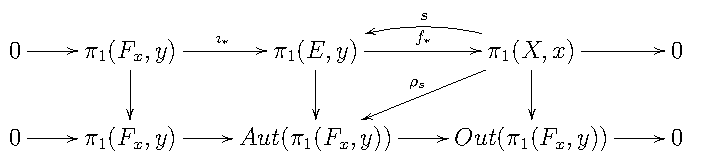
\includegraphics[width=0.5667\paperwidth]{images/L10-p086-monodromy.pdf}\end{equation}\end{figure}
平展同伦正合列也有对应的版本，即下面两个定理。
\originalnumber{1}
\begin{theorem}\label{L10S3O1}
设$f:X\to S$为平坦、固有且有限表现的概形态射，几何纤维连通且约化。假定$S$
\sourcepage{87}
连通，$\overline s:\Spec\Omega\to S$为几何点，$\overline x:\Spec\Omega\to X$为其上方的几何点。则有平展基本群正合列
\[\widehat\pi_1(X_{\overline s},\overline x)\to\widehat\pi_1(X,\overline x)\to\widehat\pi_1(S,\overline s)\to1.\]
\end{theorem}
\originalnumber{2}
\begin{theorem}\label{L10S3O2}
设$X$为域$k$上的拟紧拟分离概形，并假定$X$几何连通，即$X_{\overline k}$连通。取几何点$\overline x\in X_{\overline k}$，则存在短正合列
\[1\to\widehat\pi_1(X_{\overline k},\overline x)\to\widehat\pi_1(X,\overline x)\to\Gal(k^{\mathrm{sep}}/k)\to1.\]
\end{theorem}
沿用\eref{定理}{L10S3O2}的记号。短正合列首项$\widehat\pi_1(X_{\overline k},\overline x)$称为$X$的\textbf{几何基本群}；中间项$\widehat\pi_1(X,\overline x)$有时称为$X$的\textbf{算术基本群}。$X$的任意$k$有理点$y$给出截面$\Spec k\to X$，从而诱导截面$s_y$及同态$\rho_y$。在几何基本群无中心时，有下列交换图。
\idx{几何基本群}\idx{算术基本群}
% [Tutor Note: 原书 p87 此处作 "the first term $\widehat\pi_1(X_F,x)$"，但定理 1.2 的首项是 $\widehat\pi_1(X_{\overline k},\overline x)$，故应为 $X_{\overline k}$（$X_F$ 系笔误）；译文已作 $X_{\overline k}$。]
\begin{figure}[H]\begin{equation}\tag{3.3}\label{L10eq33}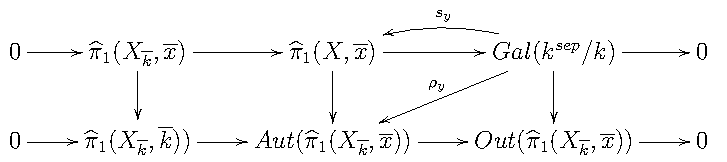
\includegraphics[width=0.5859\paperwidth]{images/L10-p087-arithmetic.pdf}\end{equation}\end{figure}
\originalnumber{3}
\begin{note}[L10S3O3]
设$A$为特征$p$的域$k$上的阿贝尔簇。当$n$与$p$互素时，$n_A:A_{\overline k}\to A_{\overline k}$为Galois有限平展覆盖，并且$\operatorname{Aut}(n_A)\cong\ker(n_A)\cong A(\overline k)[n]$。因此，当$p=0$时，
\[\widehat\pi_1(A_{\overline k},\overline0)\cong\prod_\ell T_\ell(A),\]
其中$T_\ell(A)$为$A$的Tate模。当$p>0$时，
\[\widehat\pi_1(A_{\overline k},\overline0)^{(p')}\cong\prod_{\ell\ne p}T_\ell(A).\]
对群$G$及素数$p$，$G^{(p')}$为$G$的素于$p$的完备化，即$G^{(p')}:=\varprojlim_NG/N$，逆极限遍历指数与$p$互素的正规子群$N\triangleleft G$。
\end{note}
\originalnumber{4}
\begin{note}[L10S3O4]
将光滑层$\rho_{\mathcal F}:\widehat\pi_1(X,\overline x)\to\GL(V_{\mathcal F})$限制到几何基本群$\widehat\pi_1(X_{\overline k},\overline x)$，得到与$\mathcal F$相应的几何光滑层。
\end{note}
\sourcepage{88}
\needspace{5\baselineskip}\section{第10讲参考文献}\label{L10S4}
\begin{references}
\refitem{L10bibM}{M} J. S. Milne, \emph{Lectures on étale cohomology}, Course notes. pp. 1-202. \url{http://www.jmilne.org/math/CourseNotes/CFC.pdf}.
\end{references}
